% !TEX TS-program = xelatex
% !TEX encoding = UTF-8 Unicode
% !Mode:: "TeX:UTF-8"

\documentclass{resume}
\usepackage{zh_CN-Adobefonts_external} % Simplified Chinese Support using external fonts (./fonts/zh_CN-Adobe/)
%\usepackage{zh_CN-Adobefonts_internal} % Simplified Chinese Support using system fonts
\usepackage{linespacing_fix} % disable extra space before next section
\usepackage{cite}
\setstretch{1.08} % slightly increase overall line spacing while keeping one-page layout
\geometry{left=0.9in,right=0.9in,top=0.7in,bottom=0.7in}


% \documentclass{resume}
% \usepackage{graphicx}
% \usepackage{zh_CN-Adobefonts_external}
% \usepackage{linespacing_fix}
% \usepackage{cite}



\begin{document}
\pagenumbering{gobble} % suppress displaying page number
\vspace*{\fill}

% \name{杜靖怡}

% \contactInfo{(+86) 185-3792-2003}{dujingyi7714@163.com}
% {GitHub @hijiangtao}

\noindent
\begin{tabular*}{\textwidth}{@{}p{0.22\textwidth}@{}p{0.56\textwidth}@{}p{0.22\textwidth}@{}}
    &
    \begin{minipage}[b]{0.56\textwidth}
        \centering
        {\Huge \textbf{杜靖怡}}
        
        \vspace{0.8\baselineskip}
        \mbox{\small 电话：18537922003\hspace{0.8em}邮箱：dujingyi7714@163.com}
    \end{minipage}
    &
    \begin{minipage}[b]{0.22\textwidth}
        \raggedleft
        \raisebox{-1.5\baselineskip}[0pt][0pt]{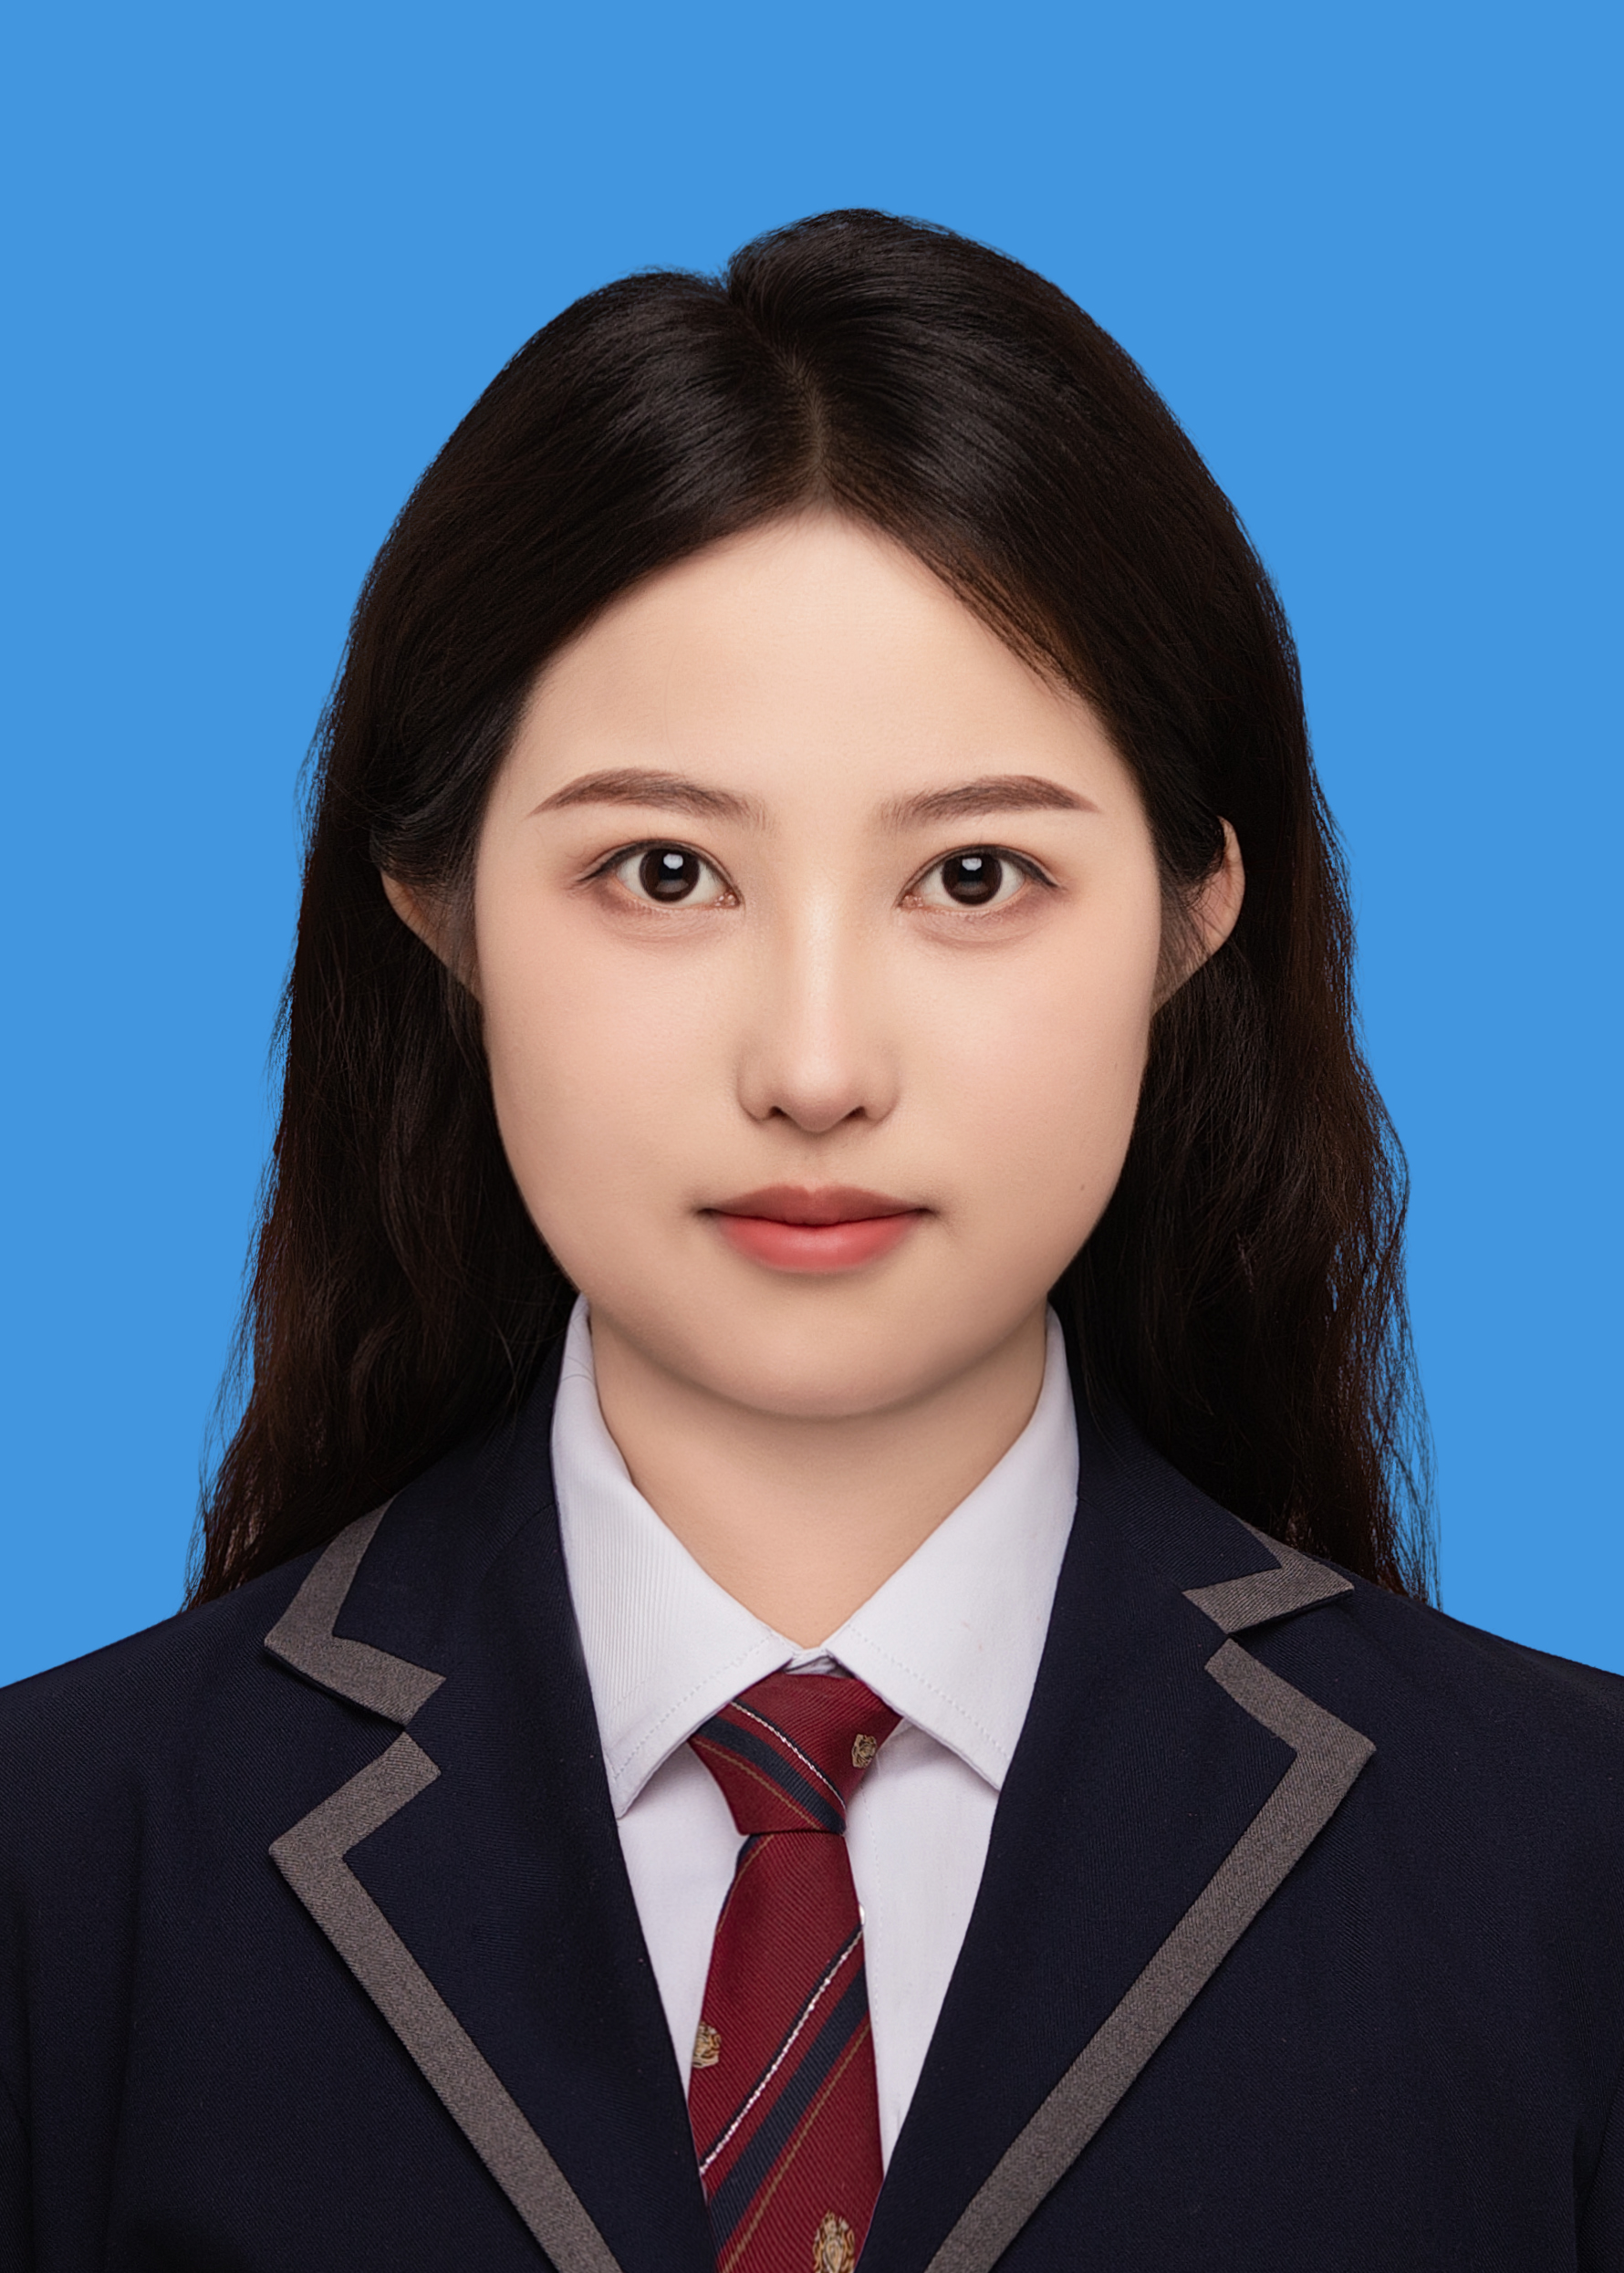
\includegraphics[width=2.5cm]{photo.jpg}}
    \end{minipage}
\end{tabular*}

\vspace{0.5\baselineskip}





\section{教育经历}

{
\renewcommand{\arraystretch}{1.25}
\begin{tabular*}{\textwidth}{@{\extracolsep{\fill}} l l l r}
\textbf{吉林大学(985)} & 统计学 & 硕士在读 & 2025.09 - 2028.06 \\
\textbf{湘潭大学(双一流)} & 统计学 & 理学学士 & 2021.09 - 2025.06 \\
\end{tabular*}
}

\vspace{-0.8em}

\begin{itemize}
    \item \textbf{GPA}: 3.34/4.0 \hfill \textbf{CET4}: 566 \hfill \textbf{CET6}: 520 \hfill \textbf{雅思}: 6.5
    \item \textbf{主修课程}：统计机器学习、深度学习、时间序列分析、运筹与优化、多元统计分析
    \item \textbf{奖项/荣誉}： 全国大学生数学建模竞赛省一、统计建模大赛省二、湖南省优秀毕业生
  
\end{itemize}

\begingroup
\setstretch{1.14}
\section{项目经历}



\datedsubsection{\textbf{多行为序列建模的 OTTO 电商推荐与用户行为预测}}{2026.05-2026.06}

\begin{itemize}

  \item 基于电商场景下用户点击、加购、下单的多行为序列，使用用户历史交互日志构建商品推荐系统，完成候选商品召回与排序任务。

  \item 设计 \textbf{Item-to-Item} 协同召回策略，利用用户历史行为构建商品共现关系，结合行为类型权重与时间衰减机制刻画用户兴趣变化，生成候选商品集合。

  \item 针对召回结果进一步构建用户-商品交互特征，融合商品侧、用户行为侧以及交互侧信息，使用 \textbf{XGBoost} 排序模型预测用户对候选商品的兴趣得分。
  
  \item 采用离线 Recall@20 指标评估推荐效果，最终 Weighted Recall@20 达到\textbf{0.541}，其中下单行为预测 Recall@20 为 \textbf{0.623}，验证了多行为序列建模对推荐效果的提升作用。
\end{itemize} 


\datedsubsection{\textbf{个人信用违约风险预测与阈值优化模型}}{2026.04-2026.05}
\begin{itemize}

  \item 针对金融风控场景中的个人信用违约识别问题，完成数据预处理与特征工程，对类别变量进行编码处理并构建信用风险预测特征。

  \item 搭建 Logistic Regression、Random Forest、SVM、GBDT、XGBoost 等多类机器学习模型，结合五折交叉验证与网格搜索进行模型选择和参数优化。

  \item 为解决类别不均衡以及高风险客户漏判问题，基于验证集搜索 \textbf{KS最大化阈值} 优化分类策略，最终测试集 AUC 达到 \textbf{0.795}，SVM 模型违约召回率由\textbf{46.7\%} 提升至\textbf{86.7\%}，显著提升了模型对高风险客户的捕捉能力。

\end{itemize}
    

\datedsubsection{\textbf{量子卷积特征提取的混合经典-量子图像分类}}{2025.11-2025.12}     

\begin{itemize}
  \item 研究量子特征增强方法在图像分类任务中的应用，基于 \textbf{PyTorch} 搭建经典 CNN 与混合经典-量子神经网络模型。设计量子特征映射方法，将图像数据编码至量子线路生成特征表示。
  \item 对比经典 CNN 与量子增强模型在 Fashion-MNIST 数据集上的分类效果，量子增强模型测试准确率达到 \textbf{82.3\%}，验证量子特征提取对图像表示学习的作用。
  
\end{itemize}

% \section{\faCogs\ IT 技能}
\section{专业技能}
% increase linespacing [parsep=0.5ex]
\begin{itemize}[parsep=0.2ex]
  \item \textbf{编程与数据处理}: 熟悉 Python、R和SQL，具备数据清洗、特征工程、实验分析和模型评估能力；了解 Git、Linux 基础操作；能够熟练使用Codex、Claude Code等AI开发工具。
  \item \textbf{机器学习与深度学习}: 掌握常见机器学习模型，熟悉交叉验证、特征选择和模型调参方法；熟悉 CNN、RNN、LSTM和Transformer 等深度学习模型结构，具备复现和调试能力。

  \item \textbf{数理统计基础}:具备扎实的概率论、数理统计、回归分析、时间序列分析和运筹优化基础，具备统计建模、预测分析和业务问题抽象能力。
\end{itemize}

% \section{\faHeartO\ 项目/作品摘要}
% \section{项目/作品摘要}
% \datedline{\textit{An Integrated Version of Security Monitor Vis System}, https://hijiangtao.github.io/ss-vis-component/ }{}
% \datedline{\textit{Dark-Tech}, https://github.com/hijiangtao/dark-tech/ }{}
% \datedline{\textit{融合社交网络数据挖掘的电视节目可视化分析系统}, https://hijiangtao.github.io/variety-show-hot-spot-vis/}{}
% \datedline{\textit{LeetCodeOJ Solutions}, https://github.com/hijiangtao/LeetCodeOJ}{}
% \datedline{\textit{Info-Vis}, https://github.com/ISCAS-VIS/infovis-ucas}{}




%% Reference
%\newpage
%\bibliographystyle{IEEETran}
%\bibliography{mycite}
\endgroup
\vspace*{\fill}
\end{document}
